 \documentclass[fleqn]{article}
\usepackage{fancyhdr} % Required for custom headers
\usepackage{lastpage} % Required to determine the last page for the footer
\usepackage{extramarks} % Required for headers and footers
\usepackage{graphicx} % Required to insert images
\usepackage{lipsum} % Used for inserting dummy 'Lorem ipsum' text into the template
\usepackage{amsmath,amsthm,amsxtra}

% Margins
\topmargin=-0.45in
\evensidemargin=0in
\oddsidemargin=0in
\textwidth=6.5in
\textheight=9.0in
\headsep=0.25in 

\linespread{1.1} % Line spacing

% Set up the header and footer
\pagestyle{fancy}
\lhead{\hmwkAuthorName} % Top left header
\chead{\courseTitle\ : \hmwkTitle} % Top center header
\rhead{\firstxmark} % Top right header
\lfoot{\lastxmark} % Bottom left footer
\cfoot{} % Bottom center footer
\rfoot{Page\ \thepage\ of\ \pageref{LastPage}} % Bottom right footer
\renewcommand\headrulewidth{0.4pt} % Size of the header rule
\renewcommand\footrulewidth{0.4pt} % Size of the footer rule

\setlength\parindent{0pt} % Removes all indentation from paragraphs

%----------------------------------------------------------------------------------------
%	DOCUMENT STRUCTURE COMMANDS
%	Skip this unless you know what you're doing
%----------------------------------------------------------------------------------------

% Header and footer for when a page split occurs within a problem environment
\newcommand{\enterProblemHeader}[1]{
\nobreak\extramarks{#1}{#1 continued on next page\ldots}\nobreak
\nobreak\extramarks{#1 (continued)}{#1 continued on next page\ldots}\nobreak
}

% Header and footer for when a page split occurs between problem environments
\newcommand{\exitProblemHeader}[1]{
\nobreak\extramarks{#1 (continued)}{#1 continued on next page\ldots}\nobreak
\nobreak\extramarks{#1}{}\nobreak
}

\setcounter{secnumdepth}{0} % Removes default section numbers
\newcounter{homeworkProblemCounter} % Creates a counter to keep track of the number of problems
\newcommand{\homeworkProblemName}{}
\newenvironment{homeworkProblem}[1][Problem \arabic{homeworkProblemCounter}]{ % Makes a new environment called homeworkProblem which takes 1 argument (custom name) but the default is "Problem #"
\stepcounter{homeworkProblemCounter} % Increase counter for number of problems
\renewcommand{\homeworkProblemName}{#1} % Assign \homeworkProblemName the name of the problem
\section{\homeworkProblemName} % Make a section in the document with the custom problem count
\enterProblemHeader{\homeworkProblemName} % Header and footer within the environment
}{
\exitProblemHeader{\homeworkProblemName} % Header and footer after the environment
}

\newcommand{\problemAnswer}[1]{ % Defines the problem answer command with the content as the only argument
\noindent\framebox[\columnwidth][c]{\begin{minipage}{0.98\columnwidth}\begin{center}#1\end{center}\end{minipage}} % Makes the box around the problem answer and puts the content inside
}

\newcommand{\homeworkSectionName}{}
\newenvironment{homeworkSection}[1]{ % New environment for sections within homework problems, takes 1 argument - the name of the section
\renewcommand{\homeworkSectionName}{#1} % Assign \homeworkSectionName to the name of the section from the environment argument
\subsection{\homeworkSectionName} % Make a subsection with the custom name of the subsection
\enterProblemHeader{\homeworkProblemName} % Header and footer within the environment
}{
\enterProblemHeader{\homeworkProblemName} % Header and footer after the environment
}

%----------------------------------------------------------------------------------------
%	NAME \longmapstoAND CLASS SECTION
%----------------------------------------------------------------------------------------

\newcommand{\hmwkTitle}{Assignment 3} % Assignment title
\newcommand{\hmwkDueDate}{February 13, 2015} % Due date
\newcommand{\courseTitle}{Physics 760} % Course/class
\newcommand{\hmwkClassInstructor}{Dr. Stefan Kycia} % Teacher/lecturer
\newcommand{\hmwkAuthorName}{John Rinehart} % Your name
\newcommand{\sudentNumber}{20503440} % Your name
\newcommand{\position}{PhD student in UWaterloo Physics department}

%----------------------------------------------------------------------------------------
%%-----------------------------------------------------------------------------------------

%%%%%%%%%%
\newcommand{\red}[1]{\textcolor[rgb]{1,0,0}{#1}}
\newcommand{\blu}[1]{\textcolor[rgb]{0,0,1}{#1}}
\newcommand{\bs}[1]{\boldsymbol{#1}}
%\newcommand{\V}[1]{\bm{#1}}
\newcommand{\V}[1]{\Vec{#1}}
\newcommand{\A}[1]{\Hat{#1}}
\newcommand{\W}[1]{\widehat{#1}}
\newcommand{\T}[1]{\widetilde{#1}}

\newcommand{\pd}[2]{\dfrac{\partial #1}{\partial #2}}
\newcommand {\ppds}[2]{\dfrac{\partial^2 {#1}}{\partial {#2}^2}}
\newcommand{\ppdss}[2]{\dfrac{\partial^2}{\partial #1 \partial #2}}
\newcommand{\pdtt}[3]{\dfrac{\partial^2 {#1}}{\partial {#2} \partial {#3}}}

\newcommand{\fpd}[2]{\frac{\partial #1}{\partial #2}}
\newcommand{\fpds}[1]{\frac{\partial}{\partial #1}}

\newcommand{\ignore}[1]{}

\newcommand{\der}[2]{\frac{d{#1}}{d{#2}}}
\newcommand{\vt}[1]{\Vec{\mathcal{#1}}}
\newcommand{\VP}[1]{\Vec{\mathbf{#1}}}
\newcommand{\vp}[1]{\mathbf{#1}}
\newcommand{\phas}[1]{\angle{#1}^{\circ}}
\newcommand{\er}{\epsilon_{r}}
\newcommand{\mr}{\mu_{r}}
\newcommand{\Lrw}{\Longrightarrow}
\newcommand{\refeq}[1]{(\ref{#1})}
\newcommand{\abs}[1]{\left| #1\right|}
\newcommand{\ket}[1]{|#1\rangle}
\newcommand{\bra}[1]{\langle #1| }
\newcommand{\intas}{\int\limits_{all\;space}}
\newcommand{\intsradial}[3]{\int\limits_{#1}^{#2} #3 r^2 \mathrm{d} r}
\newcommand{\intspolar}[3]{\int\limits_{#1}^{#2} #3 sin(\theta) \mathrm{d} \theta}
\newcommand{\intsazim}[3]{\int\limits_{#1}^{#2} #3 \mathrm{d} \phi}
\newcommand{\intcz}[3]{\int\limits_{#1}^{#2} #3 \mathrm{d} z}
\newcommand{\intcx}[3]{\int\limits_{#1}^{#2} #3 \mathrm{d} x}
\newcommand{\intcy}[3]{\int\limits_{#1}^{#2} #3 \mathrm{d} y}
\newcommand{\intavcart}[1]{\int \limits_{all\; space} #1 \, \mathrm{d} x \mathrm{d} y \mathrm{d} z}
\newcommand{\bracket}[2]{\langle#1|#2\rangle }
\newcommand*{\myalign}[2]{\multicolumn{1}{#1}{#2}}
\newcommand*\de{\mathop{}\!\mathrm{d}}

% New definition of square root:
% it renames \sqrt as \oldsqrt
\let\oldsqrt\sqrt
% it defines the new \sqrt in terms of the old one
\def\sqrt{\mathpalette\DHLhksqrt}
\def\DHLhksqrt#1#2{%
\setbox0=\hbox{$#1\oldsqrt{#2\,}$}\dimen0=\ht0
\advance\dimen0-0.2\ht0
\setbox2=\hbox{\vrule height\ht0 depth -\dimen0}%
{\box0\lower0.4pt\box2}}

%%%---
\newcommand\ointint{\begingroup
\displaystyle \unitlength 1pt
\int\mkern-7.2mu
\begin{picture}(0,3)
\put(0,3){\oval(10,8)}
\end{picture}
\mkern-7mu\int\endgroup}
%%%----
\providecommand{\abs}[1]{\lvert#1\rvert}
\providecommand{\norm}[1]{\lVert#1\rVert}

%%%%%%%%%%%%%%%

%---Packeges------------------------------------------------------------------
 %------------------------------------------------------
\usepackage{pdfsync}
\usepackage[T1]{fontenc}
\usepackage{lmodern}
\usepackage[english]{babel}
\usepackage[utf8,latin1]{inputenc}
\usepackage[T1]{fontenc}
\usepackage[usenames,dvipsnames]{pstricks}
\usepackage{epsfig}
\usepackage{pst-grad} % For gradients \usepackage{pst-plot} % For axes
\usepackage{pifont}
\usepackage{amsfonts}
\graphicspath{{IMG/}}
 \usepackage[absolute,overlay]{textpos}
 \usepackage{graphicx}
 \usepackage[bookmarks=false,pdffitwindow]{hyperref}
 \usepackage{tikz}
 \usepackage{xcolor}
 \usepackage{calc}
\usepackage{chngcntr}
\usepackage{microtype}

% Matlab code section obtained from StackExchange: http://tex.stackexchange.com/questions/75116/what-can-i-use-to-typeset-matlab-code-in-my-document
\usepackage{listings}
\usepackage{color} %red, green, blue, yellow, cyan, magenta, black, white
\definecolor{mygreen}{RGB}{28,172,0} % color values Red, Green, Blue
\definecolor{mylilas}{RGB}{170,55,241}

\lstset{language=Matlab,%
    %basicstyle=\color{red},
    breaklines=true,%
    morekeywords={matlab2tikz},
    keywordstyle=\color{blue},%
    morekeywords=[2]{1}, keywordstyle=[2]{\color{black}},
    identifierstyle=\color{black},%
    stringstyle=\color{mylilas},
    commentstyle=\color{mygreen},%
    showstringspaces=false,%without this there will be a symbol in the places where there is a space
    numbers=left,%
    numberstyle={\tiny \color{black}},% size of the numbers
    numbersep=9pt, % this defines how far the numbers are from the text
    emph=[1]{for,end,break},emphstyle=[1]\color{red}, %some words to emphasise
    %emph=[2]{word1,word2}, emphstyle=[2]{style},    
}

%----------------------------------------------------------------
\numberwithin{equation}{section}
\renewcommand{\theequation}{\arabic{equation}}



%%------------------------------------------------------------------------------------------
%	TITLE PAGE
%----------------------------------------------------------------------------------------

\title{
\vspace{2in}
\textmd{\textbf{\courseTitle\\ \vspace{0.5in}\hmwkTitle}}\\
\vspace{0.5in}\large{{\hmwkClassInstructor}}
\vspace{3in}
}
\author{\textbf{\hmwkAuthorName}\\ 
}

\date{February 6, 2015} % Insert date here if you want it to appear below your nam

%----------------------------------------------------------------------------------------
\begin{document}

\maketitle

\newpage
\tableofcontents
\newpage

%----Problems-------
\begin{homeworkProblem}
\textbf{A plane wave is incident normally from air ($n_1 =1$) on a plane slab of a transparent dielectric material with index of refraction $n_2$ and of thickness $d$. The light passes the slab and enters a third
medium with index of refraction $n_3$ and of infinite extent.}
\begin{homeworkSection}{a}
\textbf{Calculate the reflection coefficient R as a function of the thickness $d$ for monochromatic light of
wavelength $\lambda_0$ . Plot R as a function of $d$ for $n_3 =1.5$ and $n_2 =1.0, 1.2$ and  $3.0$.}
\\

As the wave travels through the medium with index of refraction $n_2$ it will acquire phase 
relative to the incident wave. Consider a wave that is incident on the slab of material 2 
at some angle $\theta_1$ relative to the normal to the surface. Some of the wave will be transmitted into material 2. This portion will have some fraction of itself reflect off the surface where 
material 3 meets material 2. If we compare the phase of the wave at the point that it 
first entered material 2 with the phase that it has when it reaches a point in its path that 
intersects the perpendicular to the initial direction of the wave when it entered material 
2 we will really be finding the phase difference between adjacent plane waves that are 
formed by reflections off material 3.
\\

To find this ``distance to the perpendicular'', consider the wave after the reflection off of 
material 3. It will first travel through 
a distance of $l_1 = \frac{d}{\cos\theta_2}$. The wave will travel another distance to reach the point where it intersects the perpendicular of the wavefront which can be shown to be 
$l_2 = \frac{d}{\cos\theta_2}\sin(\pi-(\pi/2+2\theta_2))$. Summing $l_1$ with $l_2$ and using 
some trigonometric identities, the total distance $l$ traveled through material before the 
wave reaches the ``next plane'' can be shown to be $\delta_l = 2d\cos\theta_2$. The phase 
difference between the two fictitious plane waves (the original plane wave and a time-advanced 
version of that wave is given by the $\vec{k}\cdot\vec{x}$ in the exponential describing the 
plane wave. Thus, the phase difference is $\delta_{\phi} = \frac{2\pi}{\lambda_2}\delta_l = 
\frac{4\pi}{\lambda_2}d \cos\theta_2$. In the case of normal incidence this expression 
reduces to $\delta_{\phi} = \frac{4\pi d}{\lambda_2}$.
\\

The above was necessary in order to perform the folowing steps. See, depending on the indices 
of refraction $n_1, n_2, \,\text{and}\, n_3$ the wave will reflect an infinite number of times 
between the two surfaces (where material 1 meets material 2 and, also, where material 2 
meets material 3. Each time it encounters an interface some portion of the wave will get 
reflected and some portion will be transmitted. Because of the thickness of material 2, the 
wave will also acquire a complex phase which will result in one reflected and/or transmitted 
wave's interference with all of the other instances of reflection or transmission.
\\

Consider a ray of light incident normally to the surface where materal 1 meets material 2. Assign this light a plane wave of the form $\vec{E_I}(\vec{x},t) = \vec{E_0}\exp(i(\vec{k}\cdot\vec{x}-\omega t))$. The first transmitted wave will have the form $\vec{E_{t_1}} = \vec{E_0}*t_{21}*\exp(i(\vec{k_2}\cdot\vec{x}-\omega t))*\exp(i\phi)$. $\phi$ in the previous expression accounts for the accumulation of the wave's phase as it travels though material 2 towards material 3. Note, also, that I have introduced a notation that I will use throughout the rest of this problem set. $t_{ij}$ is the scaling factor for waves which are transmitted from region j into region i. Similarly, $r_{ij}$ is the scaling factor for waves which are reflected off material j into material i. Explicit expressions for these are:

\begin{align*}
  t_{ij} &= 2\frac{n_j}{n_i+n_j} \\ 
  r_{ij} &= \frac{n_i-n_j}{n_i+n_j}
\end{align*}
\\

It is sufficient to consider just the amplitude of the wave from this point on. That is, I can safely drop the time component since I am dealing with monochromatic light and the time dependence is the same between all generated rays. The sum of all of the complex amplitudes of the transmitted rays will give me the amplitude of the resultant wave.
\\

Now, I will define a reference for the phase in this problem. The reference phase is that of the first wave immediately after it has exited the 3rd material (or, equivalently, as soon as it encounters the interface). Subsequent transmissions (due to reflections off of the interface between material 2 and material 3) will acquire a phase determined by the total distance traveled through the material. Thus, utilizing this definition and the fact that I can disregard the time component of the wave, I can express the ray that is first transmitted into material 3 as : $\vec{E}_{t_1} = \vec{E_0}*t_{21}*t_{32}$.
\\

Now, part of the incident wave makes it in the ``first pass'' to material 3. Some of this wave is reflected before any of the wave is transmitted into material 2. Some of the wave is transmitted into material 2 (this is the wave we have just considered). However, after this wave encounters material 3 a portion of this wave may be reflected at this interface. Thus, a new wave will later exit material 2 into material 3 and we must consider this wave's interference with our first wave.
\\

Utilizing the prior disussion regarding the acquired phase. I may write that the complex amplitude of the wave due to the transmission into material 1, reflections off of the two interfaces, transmission into material 3 and total distance traveled through material 2 as : $\vec{E}_{t_2} = \vec{E_0}*t_{21}*r_{23}*r_{21}*t_{32}*exp(i\frac{4\pi d}{\lambda_2}) = \vec{E}_{t_1}*r_{23}*r_{21}*exp(i\phi)$. I will omit the vector arrow above $E_0$ for brevity. I still maintain that it is a complex vector quantity. I will also allow the phase acquired due to the thickness of the plate to be designated as $\phi$. 
\\

Although we have discovered the amplitude of the second ray to penetrate material 3 we must consider that some of this ray reflected at the interface between material 2 and 3 and thus, there is a 3rd ray that will exit material 2 into material 3. Its amplitude is described by: $E_0*t_{21}*r_{23}*r_{21}*r_{23}*r_{21}*t_{23}*\exp(2 i\phi) = E_{t_2}*r_{23}*r_{21}*exp(i\phi) = E_{t_1}* (r_{23}*r_{21}*exp(i\phi))^2$.
\\

It is clear that this trend will continue ad infinitum and that the amplitude of the nth transmitted wave can be described as $E_{t_n} = E_0*t_{21}*t_{32}*(r_{23}*r_{21}*exp(i*\phi))^n$. Thus, the net wave will have an amplitude $E_t = \sum\limits_{n=0}^\infty E_0 t_{21} t_{32} (r_{23}r_{21}\exp(i\phi))^n$. This is a simple geometric series with solution $E_t = E_0 t_{21} t_{32} \frac{1}{1-r_{23}r_{21}\exp(i\phi)}$. To find the transmission coefficient T I will first normalize the transmitted wave amplitude by the incident wave. Then, I will multiply the wave amplitude by its complex conjugate. This is not complete, though. The transmission coeffecient is defined as the ratio of the transmited power per unit area and the incident power per unit area. The power per unit area is given by $\frac{1}{2}\sqrt{\epsilon}{\mu}|E_0|^2$. This can be expressed in terms of $n$ (the index of refraction of the material) as $\frac{1}{2} \sqrt{n}{c\mu}|E_0^2$. Thus, the intensity of light in the third medium divided by the intensity of light in the first medium would be given by $T = \frac{n_3}{n_1} \frac{|E_t|^2}{|E_I^2|}$.
\\

Using the previous expression and explicitly avoiding typing a lot of tedious algebra: 

\begin{problemAnswer}{
T = \frac{n_3}{n_1}|\frac{E_t}{E_0}|^2 =\frac{n_3}{n_1} \frac{(t_{21}t_{32})^2}{1-(r_{23}r_{21})^2-2 r_{23} r_{21} \cos\phi }}
\end{problemAnswer}

$\phi$ in terms of the wavelength in vacuum is $\phi = \frac{4\pi n_2}{\lambda_0}d$. I have plotted this transmission coefficient in Figure 1 as $n_2$ takes on different values. $n_1$ and $n_3$ are 1 and 1.5, respectively.

\begin{figure}
  \centering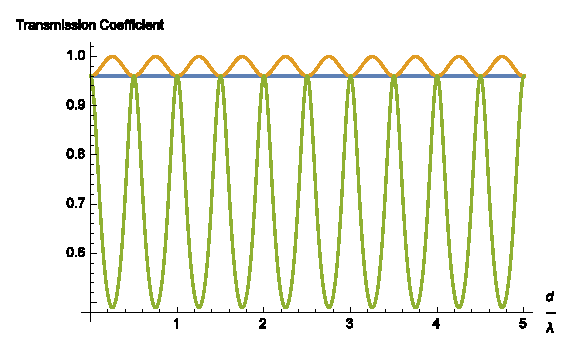
\includegraphics[width=.5\textwidth]{Images/TransCoef.eps}
  \caption{Transmission coefficient with $n_2$ = 1.5 (green), 1 (blue), 1.2 (orange) }
\end{figure}
\end{homeworkSection}

\begin{homeworkSection}{b}
\textbf{Calculate the Transmission coefficient T (transmission of incident wave into the third medium)
as a function of the thickness d for monochromatic light of wavelength $\lambda_0$ . Plot T as a function of
d for $n_3 =1.5$ and $n_2 =1.0, 1.2$ and $3.0$.}
\\

The analysis for this part of the problem will be very similar to the previous problem. The zeroth wave that is reflected will have amplitude $E_{r_0} = E_0*r_{12}$. The first wave will be related to the incident wave by $E_{r_1} = E_0*t_{21}*r_{23}*t_{12}*\exp(i\phi)$. Here, $\phi$ has the same form it did before. The second wave will have amplitude: $E_{r_2} = E_0*t_{21}*r_{23}*r_{21}*r_{23}*t_{12}*\exp(2 i\phi) = E_{r_1} * r_{21}*r_{23}*\exp(i\phi)$. The third wave will bear the same relationship with the second wave as the second wave has with the first $E_{r_3} = E_{r_2} *r_{21} * r_{23}*\exp(i\phi) = E_{r_1} * (r_{21}*r_{23})^2*\exp(2i\phi)$. Thus, it seems that the $E_{n>0}$ wave can be expressed as $E_{n} = E_{r_1}(r_{21}*r_{23}*exp(i\phi))^{n-1}$.
\\
Thus, the reflected amplitude is $E_{r} = E_{r_0} + \sum\limits_{n=1}^\infty E_{r_1}(r_{21}*r_{23}*\exp(i\phi))^{n-1}$. Recognizing the geometric series, again, and simplifying the resulting expression yields: $E_0 r_{12} + \frac{E_0 t_{21}r_{23}t_{12}\exp(i\phi)}{1-r_{23}r_{21}\exp(i\phi)}$. Taking the magnitude squared of this expression yields the reflection coefficient $R = |\frac{E_r}{E_0}|^2 = (\frac{\alpha^2 + 2 \alpha r_{12}\cos\delta\phi - 2\alpha r_{12}r_{21}r_{23}}{1+(r_{21}r_{23})^2-2 r_{21} r_{23} \cos\delta\phi} + r_{12}^2)$. $\alpha = t_{21}t_{12}r_{23}$: Substituting this into my previous expression, factoring and simplifying yields:
\begin{problemAnswer}{
R = \frac{r_{12}^2+r_{23}^2+2r_{12} r_{23}\cos\delta\phi}{1+r_{23}^2r_{21}^2-2r_{23}r_{21}\cos\delta\phi}
}
\end{problemAnswer}

I have plotted this in the second figure for the same $n_1, n_2 \,\text{and}\, n_3$ values as before for the transmission coefficient. Note that the sum of each of the corresponding plots yields 1 at any choice of the thickness of the plates.

\begin{figure}
  \centering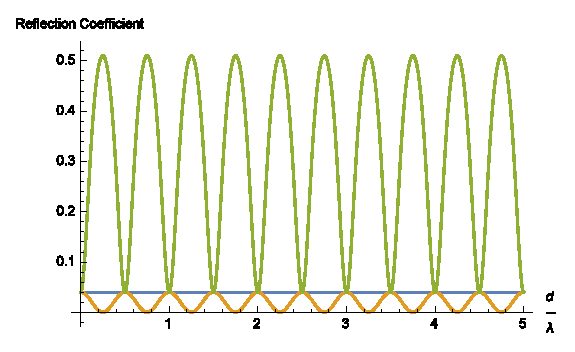
\includegraphics[width=.5\textwidth]{Images/RefCoef.eps}
  \caption{Transmission coefficient with $n_2$ = 1.5 (green), 1 (blue), 1.2 (orange)}
\end{figure}

\end{homeworkSection}

\begin{homeworkSection}{c}
An obvious application of this device is that of filtering a particular frequency of light. One could tune the distance of separation between material 1 and 3 to result in total interference in the transmission. Another application could be in using a variable distance (variable d) apparatus to experimentally determine the particular wavelength of light being generated by a monochromatic source.
\end{homeworkSection}
\end{homeworkProblem}

\setcounter{equation}{0}
---------------------
%% Problem 2
\begin{homeworkProblem}[Problem 2: Unilateral Power Spectral Density]
   \problemStatement{
In class, we examined one example with a noisy waveform $x(t)$, which is a
wide-sense statistically stationary. The autocorrelation function $
\phi_{x}(\tau) $ has a form of
\[
   \phi_{x}(\tau) = \phi_{x}(0)\exp(- \frac{|\tau|}{\tau_1})
\]
where $ \tau_1 $ is a relaxation time constant.  Compute the unilateral power
spectral density $ S_{x}(\omega) $ using the Wiener-Khintchine theorem.}

Using the Wiener-Khintchine theorem, we have:
\begin{align*}
   S_{x}(\omega) &= 4 \int_0^{\infty} \phi_{x}(0) \exp(-\frac{|\tau|}{\tau_1}) \cos(\omega
\tau) d \tau \\
&= 4 \phi_{x}(0) \int_{0}^{\infty} \exp(-\frac{|\tau|}{\tau_1}) \cos(\omega
\tau) d \tau
\intertext{Now, substituting $ \cos(\omega \tau) = .5 \left( \exp(i \omega \tau)
+ \exp(-i \omega \tau)\right) $.}
&= 2\phi_{x}(0) \int_{0}^{\infty} \exp(-\frac{|\tau|}{\tau_1}) \left( \exp(i \omega \tau)
+ \exp(-i \omega \tau)\right) d \tau \\
&= 2\phi_{x}(0) \int_{0}^{\infty} \exp(-\frac{|\tau|}{\tau_1}) \exp(i \omega \tau) d \tau +
2\phi_{x}(0) \int_{0}^{\infty} \exp(-\frac{|\tau|}{\tau_1}) \exp(-i \omega \tau)
d \tau \\
\intertext{Because the integral bounds are only over positive $ \tau $, the
absolute values signs are redundant. They will now be dropped.}
&= 2\phi_{x}(0) \int_{0}^{\infty} \exp(\frac{-\tau}{\tau_1}+i \omega \tau) d \tau +
2\phi_{x}(0) \int_{0}^{\infty} \exp(-\frac{\tau}{\tau_1}-i \omega \tau)
d \tau \\
&= 2\phi_{x}(0) \frac{\exp(\frac{-\tau}{\tau_1}+i \omega
\tau)}{\frac{-1}{\tau_1} + i\omega}\bigg|_{\tau=0}^{\infty} +
2\phi_{x}(0) \frac{\exp(\frac{-\tau}{\tau_1}-i \omega
\tau)}{\frac{-1}{\tau_1} - i\omega}\bigg|_{\tau=0}^{\infty} \\
\intertext{The upper bounds for both integrals clearly yields $ 0 $. All that
remains is the lower bound.}
&= 2\phi_{x}(0) \frac{\tau_{1}}{1-i \omega \tau_{1}} +
2\phi_{x}(0) \frac{\tau_{1}}{1 + i \omega \tau_{1}} \\
&= 2\phi_{x}(0) \frac{\tau_{1}\left( 1+ i \omega \tau_{1} \right) +
\tau_{1}\left( 1-i\omega\tau_{1}  \right)}{1+\omega^2 \tau_{1}^{2}} \\
&= 4\phi_{x}(0) \frac{\tau_{1}}{1+\omega^2 \tau_{1}^{2}}
\end{align*}
This is a Lorentzian-type function of $ \tau_1 $.
\end{homeworkProblem}

%\setcounter{equation}{0}
%--------------------- 
%\begin{homeworkProblem}

Each of three charged spheres of radius a, one conducting, one having a uniform 
charge density within its volume, and one having a spherically symmetric charge 
density that varies radially as $r^n$ (n> -3), has a total charge Q. Use Gauss's theorem 
to obtain the electric fields both inside and outside each sphere. Sketch the behavior 
of the fields as a function of radius for the first two spheres, and for the third with 
n = -2, +2. 

\begin{homeworkSection}{(a)}

Let's break the cases into different problems. The first problem is to find the electric fields over all space for a charge distribution formed by a conducting sphere of radius a. A conductor naturally spreads its static charge uniformly over the surface of the sphere. Thus, no charge resides within the sphere. Gauss' law tells us that $\oint \vec{E}\cdot \vec{da} = \frac{1}{\epsilon_0} \int_{correspondingvolume} \rho(\vec{r'})d\tau'$. Where $\rho(r')$ is the volume charge density over space. Thus, $\int_{sphere contained within the charged sphere} \vec{E} \cdot \vec{da} = 0$. This does not mean, necessarily that the electric field is zero. It only means that the amount of electric field (both negative - entering the surface - and positive - exiting the surface). However, given the symmetry of the problem at hand, all of the electric field lines will point in the radial direction. Thus, $\vec{E}\cdot \vec{da} = E A$, where A is the surface area of the sphere. However, if I were to choose a non-zero volume over which to integrate this dot product (the electric flux) then I would find that A is non-zero. However, in the interior of the sphere, there is no charge. Thus, the electric field must be zero within the interior. Outside of the shell, I have acquired all of the charge. The area of the surface over which I have performed this flux integral is $4\pi r^2$, where r is an arbitrary radius strictly larger than R, the radius of the charged sphere.
\\
Now, $\vec{E}(\vec{r})= \frac{Q}{4\pi R^2 \epsilon_0} \hat{r} H(|\vec{r}|-R)$. The Heaviside step function ``turns on'' my electric field only once my distance away from the origin, r, becomes greater than R.

Sketching this as a function of $|\vec{r}|$, I obtain the following result shown in figure \ref{chargedconductor}. In this figure I have allowed $\frac{Q}{4\pi \epsilon_0} = 1$. The horizontal axis is given in terms of $R/a$.

\begin{figure}%
\centerline{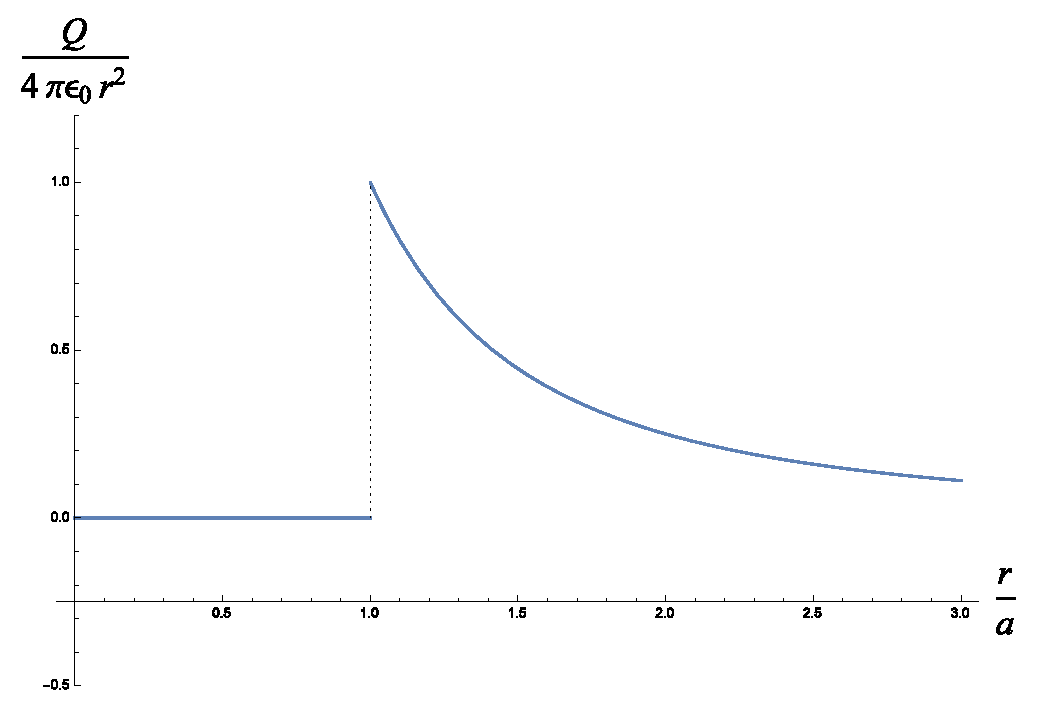
\includegraphics[width=.75\columnwidth,height=.25\paperheight]{./Images/chargedconductor.eps}}%
\caption{Magnitude of the electric field for a charged conducting sphere.}%
\label{chargedconductor}%
\end{figure}

\end{homeworkSection}

\begin{homeworkSection}{(b)}

I must attack the same problem where, now, the charge density is uniform within the volume. Now, as I integrate over the volume of the sphere I acquire charge. But, by symmetry considerations I still have a radial electric field distribution. Thus, $\oint_{area} \vec{E}\cdot \vec{da} = \frac{1}{\epsilon_0} \int_{vol} \rho(r')d\tau'$. The left hand side evaluates to $E(r) 4\pi r^2 = \rho * \frac{4}{3 \epsilon_0}\pi r^3$. This simplifies to $E(r) = \frac{\rho r}{3 \epsilon_0}$. This holds until I get outside of the charged sphere. Then, I have contained all of the charge $Q = \rho * \frac{4\pi R^3}{3}$. Thus, $E(r>R) = \frac{4\pi R^3}{3\epsilon_0} \rho \frac{1}{4\pi r^2} = \frac{\rho R^3}{3\epsilon_0 r^2}$. This is a line up until r = R. Then, the field drops off inverse quadratically. This is plotted in figure \ref{uniformsphere}. The axes and constants have been similarly scaled.

\begin{figure}%
\centerline{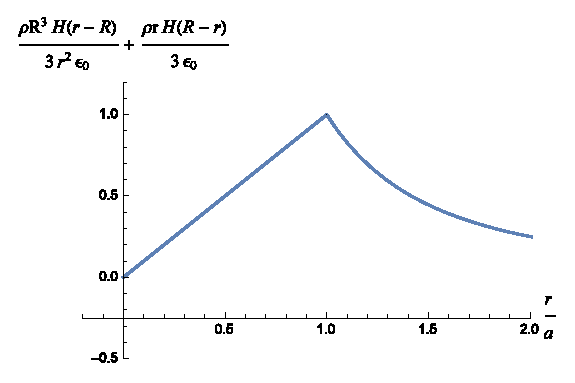
\includegraphics[width=.75\columnwidth,height=.25\paperheight]{./Images/uniformsphere.eps}}%
\caption{Magnitude of the electric field for a uniformly charged sphere.}%
\label{uniformsphere}%
\end{figure}

\end{homeworkSection}

\begin{homeworkSection}{(c)}

I must now obtain the charge distribution. I have been told that the charge density varies as $r^n$. This implies that $\rho(r) \alpha r^n H(a-|\vec(r)|)$ or that $\rho(r) = C r^n H(a-|\vec(r)|)$, where C is a normalization constant. C is constrained by the fact that $\int_{all space} \rho(r')d\tau' = Q = 4\pi C \frac{R^{n+3}}{n+3}$. Thus, $C = \frac{Q (n+3)}{4\pi R^3 R^n}$. Identifying $\frac{Q}{4\pi R^3}$ as a sort of volume density, I will assign it the label $\rho_0$. Thus, $\rho(r) = \rho_0 \frac{n+3}{R^n} r^n$; the units work. Now, skipping some algebra $E_n(r) 4\pi r^2 = \rho_0 \frac{n+3}{R^n} \frac{r^{n+3}}{n+3} 4\pi$. So, $E(r) = \rho_0 \frac{n+3}{R^n} \frac{r^{n+1}}{n+3}$. This is up until we reach the radius of the sphere. After that point, the sphere looks like a point charge. So, the field will drop off inverse quadratically.
\\
When n=2, $E_2(r<a) =  \rho_0 \frac{5}{R^5} \frac{r^{3}}{8}$. For n = -2, $E_{-2}(r<a)=\rho_0 \frac{1}{R^-3} r^{-1}$. Thus, for n=2, the field rises cubically until the boundary, then it decays quadratically. For n=-2, the field drops as inverse r until the boundary. Then, it drops off quadratically. The plots for $E_2(r)$ and $E_{-2}(r)$ are given in figures \ref{nistwo} and \ref{nisminustwo}, respetively. Similar scaling has been applied.


\begin{figure}%
\centerline{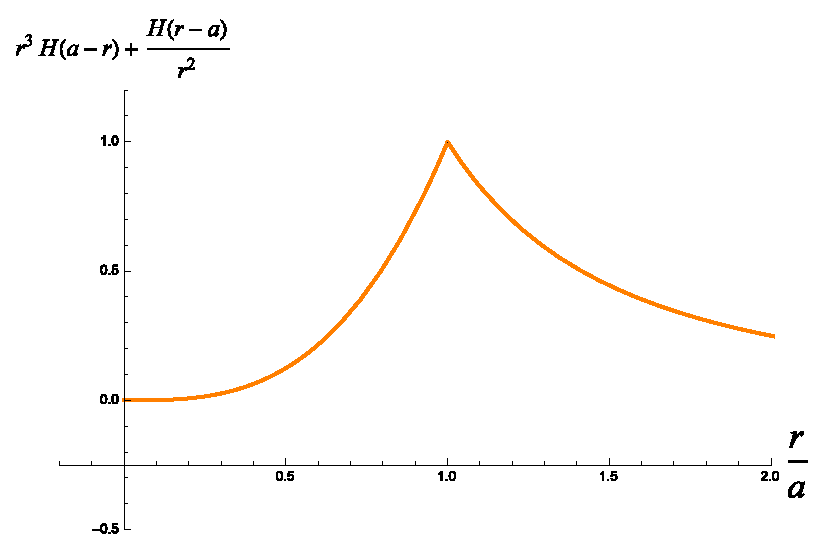
\includegraphics[width=.75\columnwidth,height=.25\paperheight]{./Images/nsphereequalstwo.eps}}%
\caption{Magnitude of the electric field for a uniformly charged sphere.}%
\label{nistwo}%
\end{figure}


\begin{figure}%
\centerline{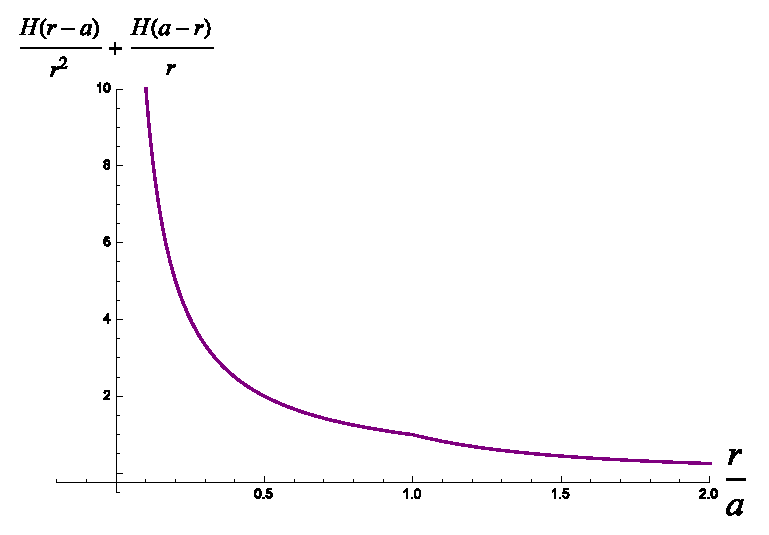
\includegraphics[width=.75\columnwidth,height=.25\paperheight]{./Images/nsphereequalsminustwo.eps}}%
\caption{Magnitude of the electric field for a uniformly charged sphere.}%
\label{nisminustwo}%
\end{figure}

\end{homeworkSection}

\end{homeworkProblem}


%\setcounter{equation}{0}
%----------------------
%%% ... %%%
%% Problem 1.4
\begin{homeworkProblem}

\textbf{Problem Description.}
\begin{align}
   \int d^{2}\alpha \ket{\alpha}\bra{\alpha} &=
   \int d^{2}\alpha
   \left( e^{\frac{-|\alpha|^{2}}{2}} \sum^{\infty}_{n=0}
   \frac{\alpha^{n}}{\sqrt{n!}} \ket{n} \right)
   \left( e^{\frac{-|\alpha|^{2}}{2}} \sum^{\infty}_{m=0}
   \frac{\bar{\alpha}^{m}}{\sqrt{m!}} \bra{m} \right)
   \intertext{Making the substition that $ \alpha \to r e^{i \theta} $ we can
   rewrite $ d^{2}\alpha $ as $ r dr d\theta $.}
   &= \int_{0}^{2\pi} \int_{0}^{\infty}
   r dr d\theta
   \left( e^{-\frac{-r^{2}}{2}} \sum^{\infty}_{n=0}
   \frac{r^{n}e^{i n \theta}}{\sqrt{n!}} \ket{n} \right)
   \left( e^{-\frac{-r^{2}}{2}} \sum^{\infty}_{m=0}
   \frac{r^{m}e^{-i m \theta}}{\sqrt{m!}} \bra{m} \right) \\
   &= \sum^{\infty}_{n=0} \sum^{\infty}_{m=0} \frac{\ket{n}\bra{m}}{\sqrt{n!}\sqrt{m!}}
   \int_{0}^{\infty} r r^{n+m} e^{-r^{2}} dr
   \int_{0}^{2\pi} e^{i\theta (n-m)} d\theta
   \intertext{But, the last integral is given by the following $ \int_{0}^{2\pi}
   e^{ia\theta} d\theta = 2\pi \delta_{a,0}$}
   &= 2 \pi \sum^{\infty}_{n=0} \frac{\ket{n}\bra{n}}{n!}
   \int_{0}^{\infty} r r^{2n} e^{-r^{2}} dr
   \intertext{Now, $ \int_{0}^{\infty} \frac{r^{2n+1} e^{-r^{2}} }{n!} dr  =
   \frac{1}{2}$. So, finally:}
   &= \pi \sum^{\infty}_{n=0} \ket{n}\bra{n}
\end{align}
\end{homeworkProblem}

%\setcounter{equation}{0}

%\begin{homeworkProblem}{Problem 5 (Jackson ed. 3 Problem 3.7)}

\begin{homeworkSection}{a}
To begin, the potential of a point charge can be expressed as \ignore{$V(\vec{r}) = k\frac{\rho(\vec{r'})}{|\vec{r}-vec{r'}} d\Tau'$} $V(\vec{r}) = k\frac{q}{|\vec{r}-\vec{r'}|}$. $\vec{r}$ is the point at which the potential is to be evaluated. $\vec{r'}$ is the point at which the charges exist. Thus, by inspection, the potential due to three point charges can be expressed as :

\[
V(\vec{r})=kq \Big(\frac{-2}{|\vec{r}|} + \frac{1}{|\vec{r} + a\hat{z}|} + \frac{1}{|\vec{r} - a\hat{z}|} \Big)
\]

To find the potential in the limiting case, let us first write $|\vec{r} + a\hat{z}|$ as $\sqrt{r^2+a^2-2ar\cos\theta}$. Here, $\theta$ is the polar angle referenced from the $+z$ axis. Doing so results in the following:

\begin{align}
V(\vec{r})&=kq \Big(\frac{-2}{r} + \frac{1}{\sqrt{r^2+a^2-2ar\cos\theta}} + \frac{1}{\sqrt{r^2+a^2+2ar\cos\theta}} \Big) \nonumber \\
V(\vec{r})&=kq \Big(\frac{-2}{r} + \frac{1}{r\sqrt{1+(a/r)^2-2(a/r)\cos\theta}} + \frac{1}{r\sqrt{1+(a/r)^2+2(a/r)\cos\theta}} \Big) \nonumber \\
\intertext{Using the following expansion (to second order) $(x^2+2\beta x +1) \rightarrow^2 1+\beta x + (1.5\beta^2-.5)r^2$} \nonumber \\
V(\vec{r})&=kq \Big(\frac{-2}{r} + \frac{1-\cos\theta (a/r) + (1.5\cos^2\theta -.5)(a/r)^2}{r} + \frac{1+\cos\theta(a/r)+(1.5\cos^2\theta-.5)(a/r)^2}{r}\Big) \nonumber \\
\intertext{Note that all terms except for the $(1.5\cos^2\theta - .5$ terms die out. But, there are two of them.} \nonumber
\end{align}

\begin{align}
V(\vec{r})&=kq \Big(\frac{(3\cos^2\theta -1)(a/r)^2}{r} \Big) \nonumber \\
\intertext{Now, according to the problem statement $qa^2 \rightarrow Q$.} \nonumber \\
V(\vec{r})&=kQ \frac{3\cos^2\theta-1}{r^3} \nonumber
\end{align}

This is already in spherical coordinates.

\end{homeworkSection}

\begin{homeworkSection}{b}
To find the solution to part (b) of this problem it will be best to do as Jackson says and use ``linear superposition to satisfy the boundary conditions''. See, the charges set up a potential at radius $r = b$. If I can find this potential I will flip its sign and slap that potential on top of the potential generated by the point charges. Whatever, potential I have in $\Phi(r,\theta,\phi)$ at $r=b$ 
due to the point charges can be used along with the potential generated by the point charges, themselves to determine the potential everywhere inside and outside of the sphere. In general, because of the problem's symmetry, my solution will be of the form : $\Theta(r,\theta) = \sum\limits_{l=0}^{\infty} A_l r^l + B_l r^{-(l+1)} P_l\cos\theta$.

The nice thing about point charges is that when that axis is located on the z-axis it is easy to express the potential due to a point charge in spherical coordinates: $\Phi(r,\theta) = \sum\limits_{l=0}^{\infty} \frac{r_<^l}{r_>^{l+1}} P_l\cos\theta$ where $r_<$ is the smaller of the following two distances: the distance from the point charge to the origin and the distance away from the origin at which the potential is being considered. This equation is valid for $\vec{r} = z \hat{z}$ and $z > 0$ (i.e. the charge is located on the positive z-axis). For charges on the negative z-axis this must be slightly modified: $\Phi(r,\theta) = \sum\limits_{l=0}^{\infty} (-1)^l \frac{r_<^l}{r_>^{l+1}} P_l\cos\theta$.

Thus, the potential due to these three point charges at $\vec{r} = b \hat{z}$ is :

\[
kQ \sum\limits_{l=0}^{\infty}\Big(\frac{a^l}{b^{l+1}} + \frac{(-1)^l a^l}{b^{l+1}}\Big) P_l\cos\theta
\]

Note that in the above all of the odd terms in the sum die because of the symmetry of the placement of the two point charges.

Note also that in the above I have chosen to ignore the potential due to the charge at the center of the coordinate system (it just shifts the above potential by a constant). If this is the potential at $r = b$ then if I flip the sign of the above potential and add it to the potential generated by the three point charges then I will effectively ground a sphere of radius b, centered at the origin. Thus, allow the ``grounded sphere'' to be constructed from both a charged sphere (with potential distribution given by the negative of the above) and the charge distribution given in the problem.

Before we set up the grounded sphere, though, let us consider what the potential inside the sphere due to the fictitious sphere looks like. For $r<b$ we can assume that because our boundary conditions (those given by the fictitious sphere) exhibit azimuthal symmetry. Thus, the potential inside the fictitious sphere looks like

\begin{center}
\[
V_{fict} = -kQ \sum\limits_{l=0}^{\infty}\Big(\frac{a^l}{b^{l+1}} + \frac{(-1)^l a^l}{b^{l+1}}\Big) P_l\cos\theta
\]
\end{center}

However, this potential must be related to the general solution for Laplace's equation inside of the sphere. Namely, these are the boundary conditions on the potential inside of the sphere.

\begin{center}
\[
	V_{fict}(b,\theta) = \sum\limits_{k=0}^{\infty}\Big(A_k b^k + B_k b^{-k+1} P_k\cos\theta \Big) = -kq \sum\limits_{l=0}^{\infty}\Big(\frac{a^l+(-1)^l a^l}{b^{l+1}}\Big) P_l\cos\theta
\]
\end{center}

If this is to hold for all $r$ (even $r=0$) then it must be the case that all $B_k$s are zero. This forces $A_k$s $=-2\frac{kq a^l}{b^{2l+1}}$. I can now write the potential within the enclosed fictitious sphere as:

\begin{center}
\[
V_{fict}(r,\theta) = (-2kq) \sum\limits_{even k=0}^\infty \frac{a^k}{b^{2l+1}} r^{-(k+1)} P_k\cos\theta
\]
\end{center}

Now, I just need to superpose this with the potential due to the point charges. The result for $|\vec{r}|>a$ is:

\[
\Phi(r,\theta) = 2kq \bigg( \sum\limits_{even k=0}^\infty a^k \Big(r^{-(k+1)}-\frac{r^l}{b^{2l+1}}\Big) P_k\cos\theta \bigg)
\]

Note that as $r \rightarrow 0$ we allow the summand to go to zero for k = 0. Thus, for small a, the largest term that survives is the $k=2$ term:

\[
\Phi_2(r,\theta) = 2kq\bigg( a^2(r^{-3} - \frac{r^2}{b^5} \bigg)P_2\cos\theta
\]

This can be seen to readily reduce to the desired expression. $k = \frac{1}{4\pi\epsilon_0}$, $Q = qa^2$.
\[ \Phi_2(r,\theta) = \frac{Q}{2\pi\epsilon_0 r^3}\bigg(1 - \frac{r^5}{b^5} \bigg)P_2\cos\theta \]

For $|\vec{r}<a|$ the potential inside the sphere only changes in the point charge term. The role of $r_<$ and $r_>$ switch. Thus, it is written:

\[
\Phi(r,\theta) = 2kq \sum\limits_{even k = 0}^{\infty} \bigg( \frac{r^k}{a^{k+1}} - \frac{a^k}{b^{2l+1}}r^{-(k+1)}\bigg) P_k\cos\theta
\]
\end{homeworkSection}

\end{homeworkProblem}
%\setcounter{equation}{0}
%\newpage
%\section{Appendix}

\subsection{Mathematica Code: Matching}
The code included in the subsection ``Mathematica Code: Matching'' provides the
Mathematica code that was used to generate the ideal match. Note that this ideal
match was not always used. In the case of the high-gain amplifier it was chosen
to reduce the gain from the maximum gain by almost as much as was possible
($\approx \SI{1}{\deci\bel}$) to ensure the lowest noise figure as was possible.
However, the results given are for those of an ideal match. To be clear, a table
is provided at the end of the section that enumerates which length of stub must
be used and what length of line (after the stub) must be used. The length of
line between the load and the stub is immaterial since the line is matched to
the load such that $Z_{in} = Z_l$.

\subsubsection{High Gain Amplifier}

\subsubsection{Low Noise Amplifier}

\subsection{MATLAB Scattering Parameter Analysis}

\subsubsection{High Gain Amplifier}

\subsubsection{Low Noise Amplifier}

%%%\newpage
%%%%-------------------------------------------
\begin{thebibliography}{9}

\bibitem{sakurai}
  J.~J.Sakurai,
  \emph{Modern Quantum Mechanics}.
  Addison Wesley, Massachusetts,
  Revised Edition.
%------------------------------------
\bibitem{greiner-relativistic_QM}
  W.~Gereiner,
  \emph{Relativistic Quantum Mechanics}.
  Springer,
  Third Edition,
  2000.
%--------------------------------------
\bibitem{taflove}
  A.~Taflove and S.C.~Hagness
  \emph{Computational Electrodynamics: The Finite Difference Time Domain Method}.
  Artech House,
  Second Edition, 2000.
  
  %----------------------------
  \bibitem{antonio004}
  A.~Soriano et.al,
  \emph{Analysis of the finite difference time domain technique to solve the Schr\"odinger's equation for quantum devices}
  Journal of App. Phys,
  vol 95,N 12,2004.
  %-------------------------------
  \bibitem{shibata}
  T.~Shibata
  \emph{Absorbing boundary conditions for the finite-difference time-domain calculation of the one-dimensional Schr\"odinger's equation}.
  Phys Rev B,
  vol 43, N 8, 1991.
  %--------------------------------------
\bibitem{kosloff}
 R.~ Kosloff and D.~Kosloff
  \emph{Absorbing boundaries for wave propagating problems}.
  Journal of Computational Phys,
  vol 63, 1986.
  %---------------------------
 \bibitem{majd}
 B.~Engquist and A.~Majd
  \emph{Absorbing boundaries for numerical solutions of the waves}.
  Math of Computation,
  vol 31, N 139, 1977. 


\end{thebibliography}


%----------------------------------------
\end{document}
